\label{sec:methodology}

In this section, we present our methodology to generate mutation tests for E2E
test programs. The methodology is illustrated in Figure \ref{fig:methodology}.
The methodology consists of the following steps:

\begin{itemize}
    
\item \textbf{Step 1:} \textit{Generating mutant:} We generate mutants with
adapted LLM models.
    
\item \textbf{Step 2:} \textit{Identifying equivalent mutants:} We use LLM
or graph methodology to identify equivalent mutants.
    
\item \textbf{Step 3:} \textit{Sorting mutants:} In this step we sort then
exclude equivalent mutants in the process. Exucluded equivalent mutants are
stored in a database for future mutant generation. We are inspired by the
Retrieval-augmented Generation (RAG)
methodology \Aurel{cite} to enrich LLM use in first step.
    
\item \textbf{Step 4:} \textit{Introducing generated mutant in PUT:} We
introduce the generated mutants in the PUT and check if PUT run successfully.

\item \textbf{Step 5:} \textit{Evaluating the generated mutants:} We evaluate
the generated mutants by checking if they are killed by the E2E test suite.
    \end{itemize}

\begin{figure}
  
    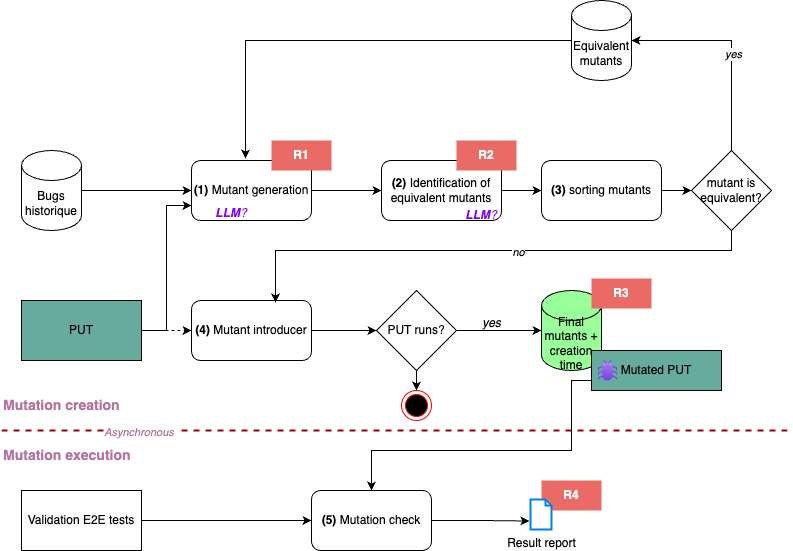
\includegraphics[width=0.5\textwidth]{figure/methodology.png}
    \caption{Methodology}
    \label{fig:methodology}
    
\end{figure}